%%%%%%%%%%%%%%%%%%%%%%%%%%%%%%%%%%%%%%%%%
%
%
%
%%%%%%%%%%%%%%%%%%%%%%%%%%%%%%%%%%%%%%%%%

%----------------------------------------------------------------------------------------
%	PACKAGES AND OTHER DOCUMENT CONFIGURATIONS
%----------------------------------------------------------------------------------------

\documentclass[
	12pt, % Default font size, values between 10pt-12pt are allowed
	%letterpaper, % Uncomment for US letter paper size
	%german, % Uncomment for German
]{fphw}

% References and Bibliography
\usepackage[hidelinks]{hyperref}
\usepackage{biblatex}
\addbibresource{bibliography.bib}

% Template-specific packages
\usepackage[utf8]{inputenc} % Required for inputting international characters
\usepackage[T1]{fontenc} % Output font encoding for international characters
\usepackage{mathpazo} % Use the Palatino font

\usepackage{graphicx} % Required for including images

\usepackage{booktabs} % Required for better horizontal rules in tables

\usepackage{listings} % Required for insertion of code

\usepackage{enumerate} % To modify the enumerate environment

\usepackage[font=small,labelfont=bf]{caption} % Required for specifying captions to tables and figures

\usepackage{placeins} % To keep floats ‘in their place’, preventing them from floating past a “\FloatBarrier” command into another section

%----------------------------------------------------------------------------------------
%	ASSIGNMENT INFORMATION
%----------------------------------------------------------------------------------------

\title{Assignment 05} % Assignment title

\author{Mélina Sladic, Lukas Probst} % Student name

\legi{XX-XXX-XXX, 22-714-240} % Legi number

\date{November 28th, 2022} % Due date

\institute{Eidgenössische Technische Hochschule Zürich} % Institute or school name

\class{Wireless Networking and Mobile Computing} % Course or class name

\professor{Dr. Mangold} % Professor or teacher in charge of the assignment

%----------------------------------------------------------------------------------------

\begin{document}

\maketitle % Output the assignment title, created automatically using the information in the custom commands above

%----------------------------------------------------------------------------------------
%	ASSIGNMENT CONTENT
%----------------------------------------------------------------------------------------

\section*{Step 2: Theory}

\begin{problem}
	What is the bandwidth of the optical spectrum (measured in Hz)?
\end{problem}
The optical or visible spectrum corresponds to a band in the vicinity of 400 to 789 THz \cite{20.500.11850/125771}.

\begin{problem}
	Is the visible spectrum regulated?
\end{problem}
There is the Federal Communications Commission (FCC\footnote{https://www.fcc.gov/licensing}) which is responsible for managing and licensing the electromagnetic spectrum for commercial users and for non-commercial users including: state, county and local governments. However, there is no regulation concerning frequency for the visible spectrum.

\begin{problem}
	What is the difference between infrared and visible light?
\end{problem}
Visible light has a wavelength that ranges from 380 nm to 750 nm on the electromagnetic spectrum while infrared light is beyond it. Infrared light has a frequency range of 300 GHz to 400 THz and a wavelenegth ranging from 700 nm to 1 mm, the beginning of the non-visible portion of the spectrum. As a result, infrared light cannot be seen by the human eye except with special technical equipment. 
\begin{figure}[!htbp] 
	\centering
	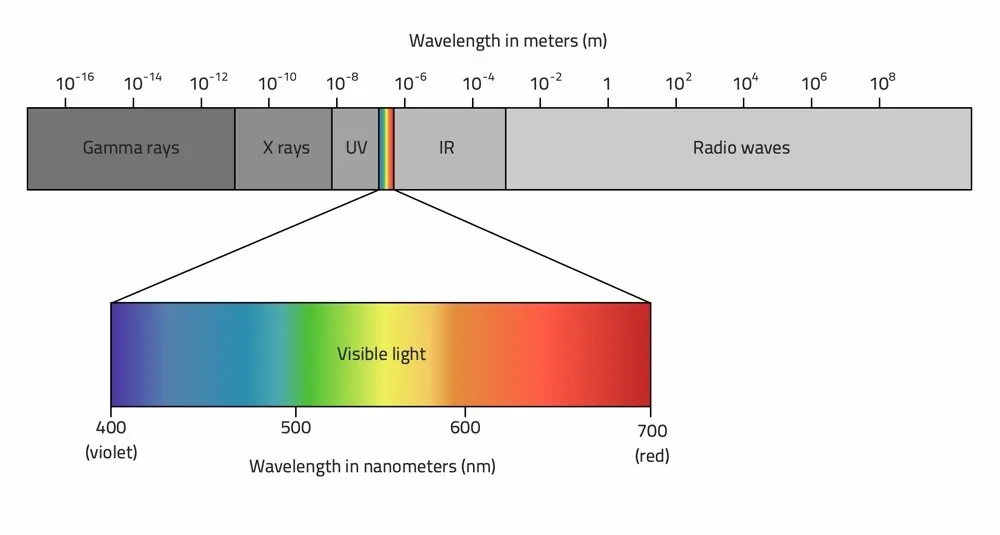
\includegraphics[width=1\columnwidth]{figures/electromagnetic_spectrum.png}
	\caption{Components of the electromagnetic spectrum.}
	\label{fig:electromagnetic_spectrum}
\end{figure}
\FloatBarrier. 

\begin{problem}
	Can infrared light penetrate water? Can visible light?
\end{problem}
Light penetrating a water surface is scattered and absorbed as it passes downward. As seen in figure \ref{fig:water_absorption}, the visible spectrum is absorbed the most in water. Within the first 10 m, water absorbs more than 50 percent of the visible light energy. Infrared light is absorbed a lot less and is therefore able to penetrate water much deeper.

\begin{figure}[!htbp] 
	\centering
	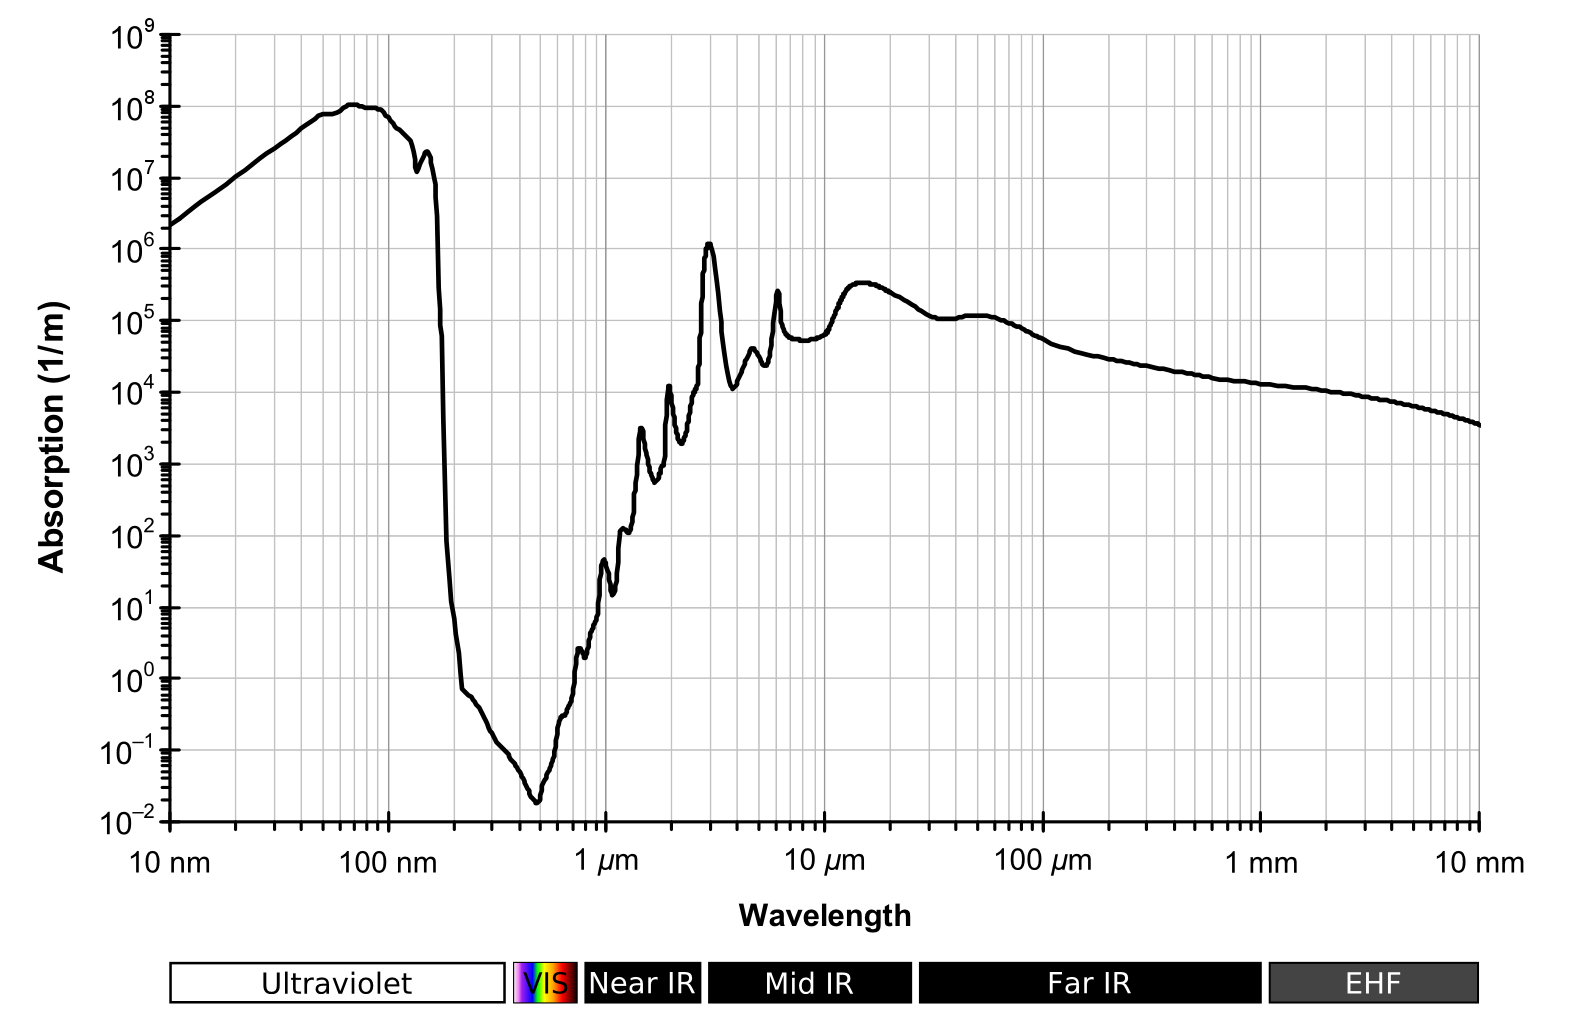
\includegraphics[width=0.75\columnwidth]{figures/water_absorption.png}
	\caption{Liquid water absorption spectrum across a wide wavelength range (image from https://en.wikipedia.org/wiki/Electromagnetic\_absorption\_by\_water).}
	\label{fig:water_absorption}
\end{figure}
\FloatBarrier. 

\begin{problem}
	What are the benefits of using an LED instead of a photodiode as a receiver in consumer electronics?
\end{problem}
The price of consumer gadgets is quite important. We do not need to include extra hardware in the form of a photodiode if the LED can still be used as a receiver. This significantly lowers costs, especially for gadgets where it is expensive to add a hole for a photodiode. Using an LED, we simply have to change the microchip without any additional costs.

%----------------------------------------------------------------------------------------

\section*{Step 3: Arduino - PC Communication}



%----------------------------------------------------------------------------------------

\section*{Step 4: Chat Application}



%----------------------------------------------------------------------------------------
\section*{Step 5: Performance Measurement at different Distances, find out the Maximum Range)}



%----------------------------------------------------------------------------------------

\clearpage
\printbibliography

\end{document}
